\section{Introduction}
\label{sec:intro}
Autonomous driving technology has achieved significant progress in perception tasks, such as 3D multiple-object tracking  (MOT) ~\cite{zhang2022mutr3d, pang2023standing, ding2024ada} and online local mapping (OLM)~\cite{droeschel2018efficient, li2022hdmapnet, liu2023vectormapnet}.  
Furthermore, autonomous systems based on Vision Language Action (VLA)~\cite{zhou2025opendrivevla, zhou2025autovla} demonstrate strong potential.
However, generic copilot systems without high-precision maps exhibit notable deficiencies in navigation, particularly in road selection and path planning under complex traffic scenarios.
A critical bottleneck hindering the navigation capability is the difficulty of collecting comprehensive road configurations. 
Acquiring specific traffic scenarios is both time-consuming and resource-intensive, often subject to geographical and regulatory restrictions. 
To address data scarcity, recent studies have leveraged diffusion models to synthesize diverse, controllable traffic scenes. 
Techniques such as BEVControl, MagicDrive, and others~\cite{yang2023bevcontrol, gao2023magicdrive, wen2024panacea, li2024drivingdiffusion, li2025dualdiff} integrate diverse conditional inputs, including text descriptions, camera parameters, and 3D spatial information, to generate traffic scenes that adhere to these controllable elements. 
These methods demonstrate the potential to generate diverse driving scenes for data augmentation and construct challenging scenarios during simulation validation.
%%%%%%元素说明
\begin{figure}[t]
	\centering
	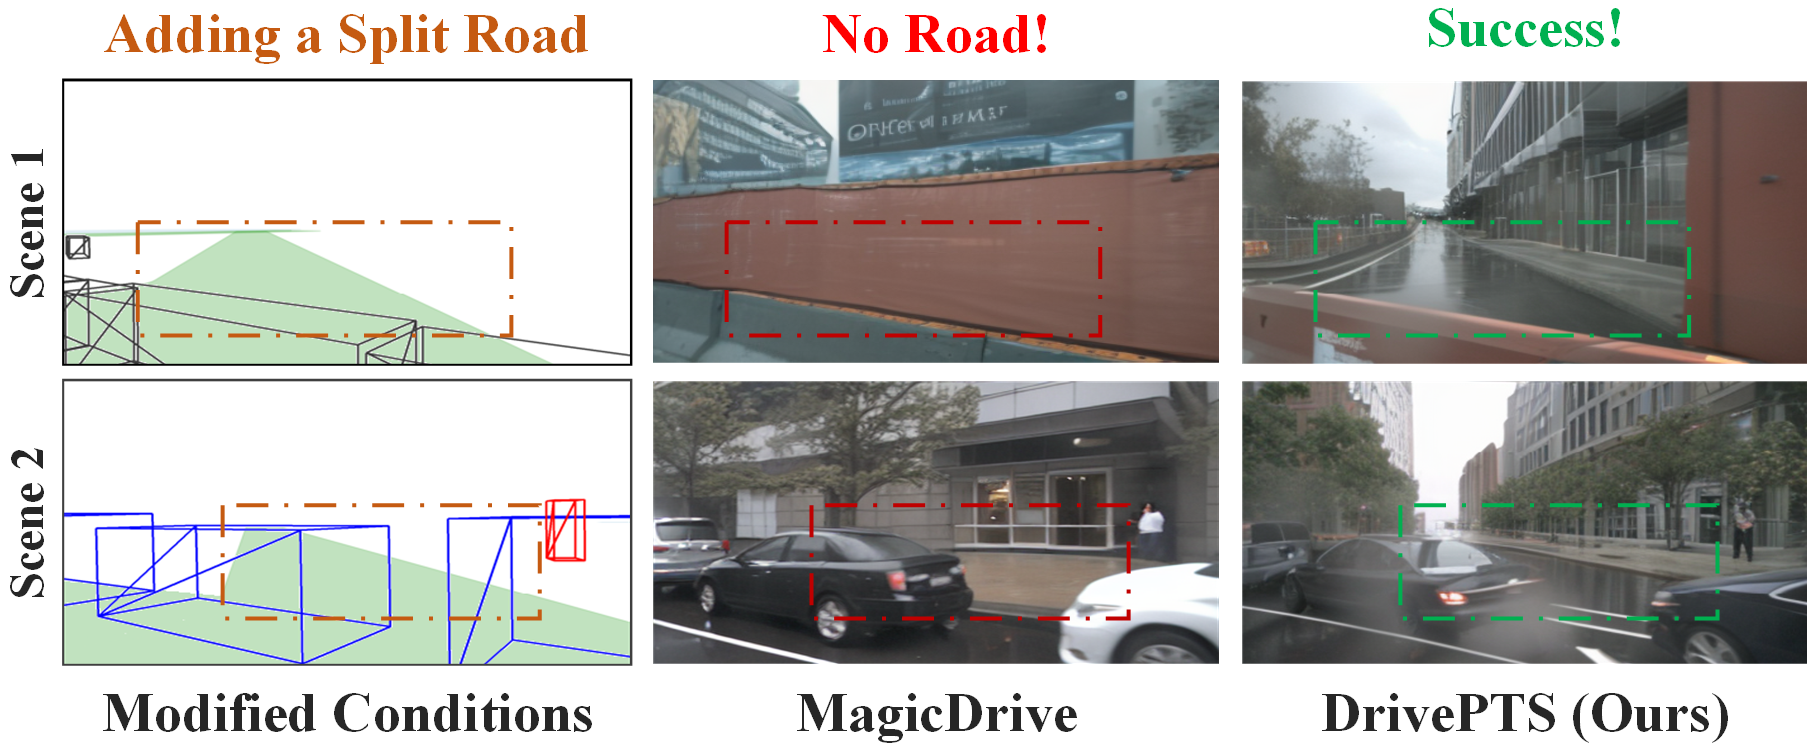
\includegraphics[width=0.465\textwidth]{split-compare-with-baselines-new.png}
	\caption{Comparison of various scene generation methods on the modified map layouts. 
		The first column highlights the modified regions of each map. 
		While MagicDrive fails to adapt to map modifications, our DrivePTS successfully generates scenes aligning with the updated map configurations.
	}
	\label{fig.0}
	\vspace{-14pt}
\end{figure}

Despite these advancements, existing methods exhibit significant limitations:
\textbf{1) Inter-dependency between geometric conditions.}
When 3D bounding boxes and maps are jointly learned, current approaches may suffer from overfitting to co-occurrence patterns between road structures and traffic objects. As illustrated in  Fig. \ref{fig.0}, the generator may implicitly associate a row of parked cars with a straight road or match roadblocks with the absence of roads, failing to produce corresponding changes even when map conditions are modified.
\textbf{2) Weak  textual guidance.}
Existing methods rely on brief, view-invariant textual descriptions that contain only basic information, failing to capture fine-grained and viewpoint-specific environmental details necessary for high-fidelity generation. 
These coarse-grained captions result in weak background modeling, as evidenced by higher Fréchet Inception Distance (FID) scores and qualitative visual assessment in our empirical studies.
\textbf{3) Lack of foreground details.}
Furthermore, existing methods prioritize global scene generation, treating all areas equally when computing the denoising loss, while neglecting foreground details. This results in structural distortions and blurriness in the generated objects and roads.


To address these challenges, we propose DrivePTS, a progressive learning framework with textual and structural enhancement for driving scene generation.
\textbf{1) Progressive learning strategy to reduce inter-condition dependency.} 
We propose a progressive training paradigm that decomposes the learning of geometric conditions. 
The model first learns to generate road layouts, followed by object placement and rendering. This separation ensures independent modeling of each condition, preventing dependencies between maps and bounding boxes. 
To mitigate catastrophic forgetting, the two phases are trained alternately. 
Once individual conditions are sufficiently learned, both are fed simultaneously for dual-input adaptation. 
Meanwhile, a mutual information constraint is also introduced to explicitly decouple the two geometric conditions.
\textbf{2) Fine-grained textual guidance via Vision-Language Model (VLM).}
We leverage a VLM to generate descriptions for each view across six distinct aspects: time, weather, road type, surroundings, objects, and spatial relationships. This multi-view, hierarchical textual guidance leads to more accurate and detailed scene generation.
\textbf{3) Foreground detail enhancement.}
We introduce a frequency-guided structure loss to strengthen the model's sensitivity to high-frequency structural elements, such as road edges and object contours, thereby mitigating  foreground distortions and blurriness.

Extensive quantitative and qualitative experiments are conducted on the nuScenes dataset~\cite{caesar2020nuscenes} to demonstrate the effectiveness of DrivePTS. Compared to recent state-of-the-art baselines, our method achieves significant improvements: FID decreases by 1.91, road IoU increases by 2.69, vehicle IoU increases by 0.69, and object detection NDS score improves by 1.44.
Visualization results show that our multi-view, hierarchical captions facilitate more comprehensive recovery of scene details, with clearer outlines of both objects and roads attributed to the frequency-guided structure loss. 
Additionally, DrivePTS can generate rare scene configurations, which existing methods fail to produce. This demonstrates the advantages of our progressive learning strategy in reducing inter-condition dependencies.
Our main contributions can be summarized:
\begin{itemize}
	\item We propose a novel progressive learning strategy that separates road and object learning into distinct stages, with a mutual information constraint to explicitly mitigate dependencies between geometric conditions.
	
	\item We develop a VLM-driven approach to generate multi-view hierarchical descriptions across multiple semantic dimensions, providing fine-grained textual guidance that enhances scene generation fidelity.
	
	
	\item A frequency-guided structure loss is introduced to improve structural fidelity by enhancing the model's sensitivity to high-frequency components.
\end{itemize}

